\documentclass[a4paper]{report}
\usepackage[utf8x]{inputenc}
\usepackage[T1]{fontenc}
\usepackage[french]{babel}
\usepackage{graphicx}
\usepackage{footmisc}
\usepackage{fullpage}
\usepackage{eso-pic}
\usepackage{hyperref}
\usepackage{textcomp}
\usepackage{float}
\usepackage{appendix}
\usepackage{amsthm}
\usepackage{amsmath}
\usepackage{listings}
\usepackage{color}
\usepackage{subcaption}



\usepackage{array}

\definecolor{codegreen}{rgb}{0,0.6,0}
\definecolor{codegray}{rgb}{0.5,0.5,0.5}
\definecolor{codepurple}{rgb}{0.58,0,0.82}
\definecolor{backcolour}{rgb}{0.95,0.95,0.92}

\lstdefinestyle{mystyle}{
    backgroundcolor=\color{backcolour},
    commentstyle=\color{codegreen},
    keywordstyle=\color{magenta},
    numberstyle=\tiny\color{codegray},
    stringstyle=\color{codepurple},
    basicstyle=\ttfamily\footnotesize,
    breakatwhitespace=false,
    breaklines=true,
    captionpos=b,
    keepspaces=true,
    numbers=left,
    numbersep=5pt,
    showspaces=false,
    showstringspaces=false,
    showtabs=false,
    tabsize=2
}



\lstset{style=mystyle}
%\renewcommand{\thesection}{\arabic{section}}

%%\renewcommand\lstlistingname{Quelltext} % Change language of section name

%\providecommand{\tightlist}{%
%temsep}{0pt}\setlength{\parskip}{0pt}}

\providecommand{\tightlist}{}

\newcommand{\HRule}{\rule{\linewidth}{0.5mm}}
\newcommand{\blap}[1]{\vbox to 0pt{#1\vss}}
\newcommand\AtUpperLeftCorner[3]{%
  \put(\LenToUnit{#1},\LenToUnit{\dimexpr\paperheight-#2}){\blap{#3}}%
}
\newcommand\AtUpperRightCorner[3]{%
  \put(\LenToUnit{\dimexpr\paperwidth-#1},\LenToUnit{\dimexpr\paperheight-#2}){\blap{\llap{#3}}}%
}

\title{\LARGE{\begin{center}MÉMOIRE DE STAGE\end{center} \leavevmode\newline Résolution de Sudoku}}
\author{\textsc{Minatchy} Jérôme\\M1 Informatique\\Année universitaire 2020/2021 à rendre pour le 3 Juin 2021}
\date{\today}
\makeatletter

\begin{document}
\begin{titlepage}
    \enlargethispage{2cm}

    \AddToShipoutPicture{
        \AtUpperLeftCorner{1cm}{0.5cm}{
\includegraphics[width=4cm]{./images/logoUA.jpg}}
    }
    \begin{center}
        \vspace*{1cm}
        
\includegraphics[width=6.5cm]{./images/lamialogo.jpg}
        \vspace*{0.5cm}

        \textsc{\@title}
        \HRule
        \vspace*{0.5cm}

        \large{\@author}
    \end{center}

    \begin{center}
      \vspace*{2cm}
      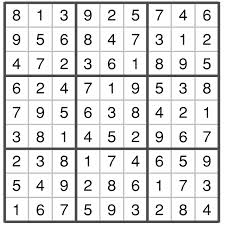
\includegraphics[width=6.5cm]{./images/sudoku1.jpeg}
    \end{center}

    \vspace*{2cm}

    \begin{center}
        Université des Antilles

        (Entreprise d'accueil)
        %\makebox[\textwidth]{
\includegraphics[width=\paperwidth]{./images/logoUA.jpg}}
    \end{center}

\end{titlepage}
\ClearShipoutPicture

\listoffigures
\tableofcontents

\hypertarget{Introduction}{%
\chapter{Introduction}\label{Introduction}}

\chapter{Présentation du métier de Data Scientist}

\section{Intitulé du métier}

Généralement rattaché à la direction des systèmes d'information (DSI) d’une entreprise, le Data Scientist a pour objectif d’analyser et d’exploiter toutes les datas des clients, des prospects ou bien encore des employés que l’entreprise récupère via différents canaux. L’objectif est de créer des modèles prédictifs et d’aider la prise de décision par la construction d'algorithmes.

\section{Contenu de l'activité  }
\begin{itemize}
\item Définir les méthodes et les outils de traitement de l'information
\item Réaliser des veilles documentaires (collecte, analyse etc.)
\item Réaliser des études
\item Rédiger l'information produite (études, synthèses, rapports, bulletins, ...) et établir des prévisions, des évaluations, des recommandations, des perspectives, ...
\item Adapter les outils de traitement statistique de données
\item Présenter et diffuser les résultats des études réalisées
\end{itemize}

\section{Formation nécéssaire}
Pour se spécialiser : des écoles d’ingénieurs avec des filières mathématiques appliquées ou statistiques ou des formations spécialisées en big data : Centrale Supélec, l'École polytechnique, Télécom Paris, le CNAM, l'ENSIMAG (Grenoble), etc. Des masters universitaires spécialisés informatique, data ou statistique, des MBA big data d’écoles de commerce.

\section{Qualités requises}
\begin{itemize}
\item Esprit critique
\item Communication efficace
\item Approche proactive de la résolution des problèmes
\item Curiosité intellectuelle
\end{itemize}

\newpagepp

\section{Lieux d'exercice}
\begin{itemize}
\item Collectivité territoriale
\item Entreprise
\item Établissement/organisme de recherche
\item Organisme d'études et de sondage
\item Organisme de crédit
\item Organisme professionnel
\item Société de conseil
\item Société de services
\end{itemize}

\section{Interrogations personnels}
\begin{itemize}
\item Est-il mieux d'avoir un master en mathématique qu'un master informatique pour exercer ce métier?
\item L'intelligence artificiel aura t-elle une place inmportante dans ce métier ?
\end{itemize}

\chapter{Expériences professionnels}

\section{Tableaux des expériences}

\begin{tabularx}{15cm}{|X|X|X|}
\hline \rowcolor{lightgray}
In this table & each column got the same & width\\
\hline
In this table & each column got the same & width\\
\hline
\multicolumn{3}{|l|}{texte de la case} \\
\hline
\multicolumn{3}{|l|}{texte de la case} \\
\hline
In this table & each column got the same & width\\
\hline
\end{tabularx}

\section{Bilan des compétences par type d'expérience}

\begin{tabularx}{15cm}{|X|X|X|X|X|}
\hline
\rowcolor{color1}
 & Stage & Projets & Jobs & Associations\\
\hline
Savoir & Connaître les outils de  dévellopements et programation actuels & Connaitre les principales nouveauté en matière d'IA et d'optimisation & Aucun & Aucun\\
\hline
Savoir faire & Utiliser les outils de  dévellopements et programation actuels & Orgniser et prévoir les taches d'un projet & Aucun & Aucun\\
\hline
Savoir être & Autonomie & Diplomatie & Aucun & Aucun\\
\hline
\end{tabularx}

\section{Synthèse sur la maîtrise et
la satisfaction des compétences}

\begin{tabularx}{15cm}{|X|X|X|}
\hline
\rowcolor{color1}
Compétence & Maîtrise & Satisfaction\\
\hline
 Connaître les outils de  dévellopements et programation actuels & Moyenne & Non satisfait\\
\hline
Utiliser les outils de  dévellopements et programation actuels & Moyenne & Non satisfait\\
\hline
Connaitre les principales nouveauté en matière d'IA et d'optimisation & Moyenne & Non satisfait\\
\hline
Orgniser et prévoir les taches d'un projet  & Moyenne & Non satisfait\\
\hline
\end{tabularx}

\section{Différentiel de compétences entre les
attentes de l’employeur et vos compétences}

\begin{tabularx}{15cm}{|X|X|X|X|}
\hline
\rowcolor{color1}
Compétence & Maîtrise & Satisfaction & Écart\\
\hline
 Connaître les outils de  dévellopements et programation actuels & Moyenne & Non satisfait & Moyen\\
\hline
Utiliser les outils de  dévellopements et programation actuels & Moyenne & Non satisfait & Nul\\
\hline
Connaitre les principales nouveauté en matière d'IA et d'optimisation & Moyenne & Non satisfait & Moyen\\
\hline
Orgniser et prévoir les taches d'un projet  & Moyenne & Non satisfait & Fort\\
\hline
\end{tabularx}

\hypertarget{conclusion}{%
\chapter{Conclusion}\label{conclusion}}

\section{Rappel de la problèmatique}

Notre problèmatique à la base était la résolution de sudoku Standart ce que nous avons reussi. Nous avons donc pour avoir une autre vision du problème nous avons choisi de généraliser celui-ci. Ce qui nous a ouvert à des pistes d'améliorations dont nous n'aurions pas eu besoin dans le cas de la résolution de sudoku standart.

\section{Réponse apportées}
Nous avons en ce qui concerne la résolution de sudoku standart deux programmes permettant leurs résolution quand aà la généralisation de ceux-ci nous avons un programes parfaitement fonctionnel permettant sa résolution via Cplex.
\section{Piste d'amélioration}
Nous pourrions pour voir les limites de l'algorithme du Cplex l'utiliser sur un grand volume de sudoku et voir le temps mis pour tous les résoudre en une seule fois. Nous pourrions essayer avec des sudokus d'une taille extrème pour en vérifier la consistence.\newline Comme dit précédemment en ce qui concerne la déduction des valeurs nous pouvons éviter beaucoup de test inutiles grace à cela pour amélioré notre algorithme utilisant le backtracking.\newline
Nous pouvons aussi pour les tests sur les sudokus de taille standart tester nos algorithme sur les classes de sudoku décrite dans cette article:\newline
\cite{Differents}
\newline
Nous expliquant que tout les sudoku possibles peuvent être obtenu par plusieurs actions élémentaires à partir de 5472730538 grilles de sudoku que nous pouvons qualifier d'élémentaires.
Cela nous permettrait d'affirmer de manière solide que nos algorithme fonctionnent dans tout les cas possibles.

\section{Les apports du stage}

\subsection{les apports à l'entreprise}
Grace à ce Stage les chercheurs auront une meilleur idée de l'utilisation de Cplex sur python pour la résolution de leurs problèmes et grace à notre algorithme utilisant le backtracking nous pouvons appuyer que l'utilisation des algorithmes de Cplex est bien plus efficaces que les méthodes que nous pouvons coder de façon artisanal sans y consacrer une très grande quantité de connaissances.

\subsection{les apports personels}

Avant ce stage je n'avais aucune connaissance en résolution de problème d'optimisation linéaire. Grace à ce stage je connais maintenant un de ses outils de résolution les plus puissant. J'ai aussi pu apprendre plusieurs termes de mathématique combinatoire que je n'aurais jamais connu autrement. J'ai maintenant la connaissance de plusieurs algorithme de résolution de problème de satisfaction de contrainte. J'ai nmaintenant aussi les connaissances basique nécéssaire quant à la programmation d'interface graphique avec Qt.



\cleardoublepage
\phantomsection
\bibliographystyle{plain} % Le style est mis entre accolades.
\addcontentsline{toc}{chapter}{Bibliographie}
\bibliography{biblioMinatchy}


\appendix


%\include{bases}

\end{document}
